\renewcommand{\theequation}{\theenumi}
\begin{enumerate}[label=\arabic*.,ref=\thesubsubsection.\theenumi]
\numberwithin{equation}{enumi}

\begin{figure}[!ht]
\centering
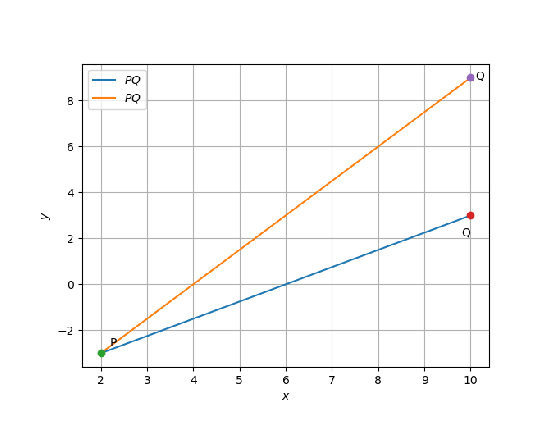
\includegraphics[width= \columnwidth]{./figs/line/point_vec/point_vec.eps}
\end{figure}

 \item The distance between two points is given by equation
 \begin{align}
 \brak{\vec{P}-\vec{Q}}^T\brak{\vec{P}-\vec{Q}}=10^2\\
 \brak{\vec{P}^T-\vec{Q}^T}\brak{\vec{P}-\vec{Q}}=100\\
 \norm{P}^2 - \vec{P}^T\vec{Q} - \vec{Q}^T\vec{P} + \norm{Q}^2 = 100
 \end{align}
 On substituting 
 \begin{align}
 y^2 + 6y -27 &= 0\\
 \brak{y+9}\brak{y-3} &= 0
 \end{align}
 The roots of the above quadratic equation are -9 and 3. Therefore the values of y = -9,3

\item Both the lines in the graph have length equal to 10 units. $ \vec{Q}$ can have two values $ \myvec{10 \\3}$ and $ \myvec{10 \\-9}$.

\item The python code to find the roots of the quadratic equation can be downloaded from
\begin{lstlisting}
codes/line/point_vec/roots.py
\end{lstlisting}
\item The python code for the figure can be downloaded from
\begin{lstlisting}
codes/line/point_vec/point_vec.py
\end{lstlisting}


 
 \end{enumerate}